\chapter{Literature Review}\label{lreview}
\section{Overview}\label{lroverview}
As we've mentioned in previous chapter, OkNN problem appears in both
AI path planning and Spatial query processing. Therefore, this literature review includes
related works in these two fields.

In section~\ref{lrai}, we introduce two classic pathfinding algorithms:
\textit{Dijkstra} and \textit{A*}, as the historic background.
In section~\ref{lrindex}, we introduce a spatial index \textit{R-tree},
and discuss how it solves traditional kNN problem.
In section~\ref{lrknn}, we focus on existing works on OkNN, two algorithms based on
\textit{Local Visibility Graph} will be discussed. 
In section~\ref{lrnav}, we introduce a very fast point-to-point algorithm in AI path planning
field which shows a new direction to solve OkNN problem.
In section~\ref{lrquery}, we briefly discuss other related spatial queries which can be
improved by our research.

\section{Classic pathfinding}\label{lrai}
The most widely used pathfinding algorithm is \textit{Dijkstra} \cite{dijkstra1959note}. 
The algorithm works on a nonnegative weighted graph, it requires a priority queue and
regards the length of shortest path as key, and it visit vertices in the order
of lenght of shortest path until requirements be satisfied, e.g. the target has been found.
When the target is the furthest vertex to the start vertex, \textit{Dijkstra} has to explore the entire
map. Based on such consideration, researchers generalized \textit{Dijkstra} algorithm to
\textit{best-first search} which explores a graph by expanding the most promising node chosen
acording to a specified rule.
\textit{A*} \cite{hart1968formal} is known as a famous \textit{best-first search},
it select the path that minimizes:
$$
f(n) = \textit{g-value}(n) + \textit{h-value}(n)
$$
where $n$ is the last node on the path, \textit{g-value} is the length of shortest path from start to
$n$, \textit{h-value} is a estimation of shortest path from $n$ to the goal which is
problem-specific. One important propert of \textit{h-value} is admissibility, meaning that it never
overestimates the actual cost to the target.
For example, in an Euclidean plane with obstacles, \textit{h-value} can be the Euclidean
distance.

In following sections and the chapter~\ref{proposedalgo}, we will show how \textit{Dijkstra} and
\textit{A*} algorithms be applied on the OkNN problem.

\section{Spatial Index}\label{lrindex}

\subsection{\textit{R-tree}}

\textit{R-tree} has many variations\cite{guttman1984r,beckmann1990r,sellis1987r+,kamel1993hilbert},
they improve efficiency in different aspects,
but they still provide same functionality,
so we only introduce the classic \textit{R-tree} in this section.

\begin{figure}[htp]
  \centering
  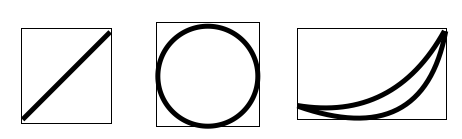
\includegraphics[width=.8\linewidth]{pic/mbr.PNG}
  \caption{\small Both segments, circle and irregular shape can be represented by their MBR}
  \label{mbr}
\end{figure}

\textit{R-tree} is a heighb-balanced tree \cite{guttman1984r}, all objects are stored in leaf
node. In leaf node, if an object is not a point, it would be represented by its \textit{Minimal Bounding
Rectangle} (MBR), figure~\ref{mbr} shows example of MBRs. Each interior node is also
represented by a MBR which contains either leaf nodes or descendant interior nodes.
To guarantee efficiency, each non-root node of \textit{R-tree} can contain at least $m$ entries
and at most $M$ entries, where $m, M$ are specified constant when \textit{R-tree} is built, and
\textit{R-tree}'s root alway has two entries. 
Usually, objects retrieval start from the root,
then narrow down to children nodes based on spatial information in their MBRs, and finally
retrieve objects from leaf nodes.
Figure~\ref{rtree} shows how to store and retrieve objects.

\begin{figure}[htp]
  \centering
  \begin{subfigure}{.5\textwidth}
    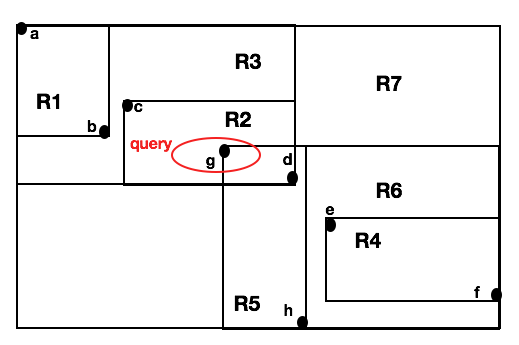
\includegraphics[width=\linewidth]{pic/hierarchy_mbr.PNG}
    \caption{Hierachy of MBRs}
    \label{hmbr}
  \end{subfigure}%
  \begin{subfigure}{.5\textwidth}
    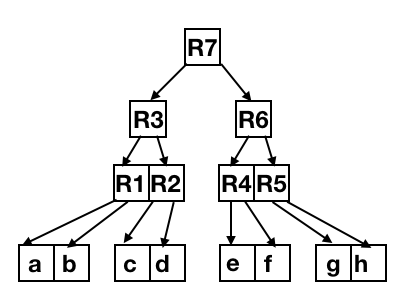
\includegraphics[width=\linewidth]{pic/rtree.PNG}
    \caption{Corresponding tree structure}
    \label{tree}
  \end{subfigure}
  \caption{\small $\{a,b,c,d,e,f,g,h\}$ is the object set,
  $R1,R2,R4,R5$ are leaf nodes, $R3,R6$ are interior nodes, and $R7$ is the root.
  The red oval is a range query, starting with $R7$, since $R6$'s MBR overlapped with query
  area, we narrow down to $R6$, then to $R5$, and finally retrieve $g$. Notice that $R3,R2$ also
  overlap with the query, so they will also be visited, but nothing retrieved.
  }
  \label{rtree}
\end{figure}

From the example in figure~\ref{rtree}, we can see that overlapping area will be explored
multiplel times in retrieval progress, which duplicated efforts.
So there is a variant doesn't allow overlapping in interior node, called $R^+\textit{-tree}$\cite{sellis1987r+}.

\subsection{Nearest Neighbor Query}
In the \textit{R-tree}, all nodes are organized by their spatial information,
so that the nearest neighbor of a point can be retrieved by exploring tree nodes in some order.
To introduce the algorithm, we need to discuss two metrics: given query point $q$ and the MBR of a tree node
\begin{itemize}
  \item \textit{\textbf{mindist}} is the minimal distance from $q$ to the MBR, it estimates the
    distance from $q$ to inside object, so this metric is the priority of the tree node;
  \item \textit{\textbf{minmaxdist}} is the uppber bound of the NN distance of any object inside
    the MBR, if the $mindist$ of any MBR large than this value, then such MBR cannot contains
    the nearest object, so this metric is for pruning.
\end{itemize}
The algorithm starts with root node and proceeds down the tree. When it visits a leaf node,
current nearest neighbor will be updated;
When it visits a non-leaf node, the children of such node is sorted by \textit{mindist}, and pruned by
\textit{minmaxdist}; when algorithm finished, the updated nearest neighbor is the answer.  
This kind of algorithm is also called \textit{branch-and-bound} traversal, which has been well
studied and widely used in other artifical intelligence areas\cite{sellis1987r+},
and existing NN queries based on it with different ordering and pruning strategies,
more details are in \cite{roussopoulos1995nearest,cheung1998enhanced}.

\section{Obstacle k-Nearest Neighbor}\label{lrknn}
\section{Pathfinding on Navigation Mesh}\label{lrnav}
\section{Related Spatial Queries}\label{lrquery}
